Given a random sample $\prth{X}{i}{1}{n}$ from a population $X$ with 
probability distribution $f(x;\theta)$ where $\theta$ is a parameter, a 
statistics is a function $T$ of $\prth{X}{i}{1}{n}$ that is:
$$
T = T\left( \prth{X}{i}{1}{n} \right)
$$
\section{Monte Carlo approximation}
In general, computing the distribution of a function of a random variable using the change
of variables formula can be difficult. One simple but powerful alternative is to generate 
$S$ samples from distribution, one popular method for higher dimensional distributions, is
called Markov chain Monte Carlo or MCMC.
Given the samples we can approximate the distribution of $f(X)$ by using the empirical 
distribution of $\left\{f(x_{s})\right\}^{S}_{s=1}$
We can varying many quantities such as:
\begin{itemize}
	\item $\E{X} \rightarrow \overline{x} = \dfrac{1}{S}\su{{s=1}}{S}x_{S}$ 
	\item $\V{X} \rightarrow \dfrac{1}{S}\su{{s=1}}{S}(x_{s}-\overline{x})^{2}$
	\item $\Prob{X\leq c} \rightarrow \dfrac{1}{S}Card(\left\{x_{s}\leq c\right\})$
	\item $ median(X) \rightarrow median(\left\{x_{i}\right\}_{1\leq i\leq S})$
\end{itemize}

\section{Chi-Square distribution}
\paragraph{Definition}
A continuous variable $X$ is said have a Chi-Square distribution with
$r$ degrees of freedom if its probability density function is of the form
$$
f(x;r)=
\left\{
\begin{array}{ll}
\dfrac{1}{\Gamma\left(\frac{r}{2}\right)^{2^{\frac{r}{2}}}}x^{\frac{r}{2}-1}e^{-\frac{x}{2}} & \mbox{if } 0 \leq x\leq \infty \\
0 & \mbox{otherwise}
\end{array}
\right.
$$
Recall that a gamma distribution reduces to Chi-Square distribution if 
$\alpha = \frac{r}{2}$ and $\theta = 2$.
\begin{figure}[H]
	\begin{center}
		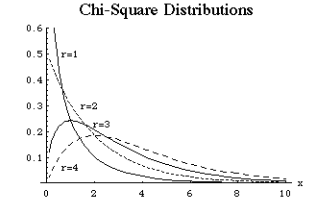
\includegraphics[width=\textwidth]{./chaps/23sec/images/1chi_square.png}
	\end{center}
	\caption{If $r\rightarrow\infty$ then chi-square distribution
	tends to normal distribution}
	\label{fig:23sec_chiSquared}
\end{figure}

\paragraph{Properties}
\subparagraph{Population}
If $X\hookrightarrow N(\mu, \sigma^{2}) \text{, then }\left( \frac{X-\mu}{\sigma} \right)^{2}\hookrightarrow\chi^{2}(1)$
\subparagraph{Sample} If $X\hookrightarrow N(\mu,\sigma^{2})\text{ and }\prth{X}{i}{1}{n}$ is a random sample from $X$, then:\\
$$ \su{{i=1}}{n}\left( \dfrac{X_{i}-\mu}{\sigma} \right)^{2}\hookrightarrow\chi^{2}(n)$$
\subparagraph{Sample variance} If $X\hookrightarrow N(\mu,\sigma^{2})\text{ and }\prth{X}{i}{1}{n}$ is a random sample from $X$, then:\\
$$ \dfrac{(n-1)S^{2}}{\sigma^{2}}\hookrightarrow\chi^{2}(n-1)$$
\subparagraph{Gamma} IF $X\hookrightarrow \gamma(\theta,\alpha)$, then:
$$ \dfrac{2}{\theta}\hookrightarrow\chi^{2}(2\alpha)$$

\section{Student's t-distribution}
\paragraph{Definition}
A continuous random variable $X$ is said to have a $t$-distribution 
with $\nu$ degrees of freedom if its probability density function is of
the form:
$$
f(x;\nu) = 
\dfrac{\Gamma\left(\frac{\nu+1}{2}\right)}{\sqrt{\pi\nu}~\Gamma\left(\frac{\nu}{2}\right)\left(1+\frac{x^{2}}{\nu}\right)^{\left(\frac{\nu+1}{2}\right)}}, -\infty\leq x\leq\infty
$$
where $\nu > 0$. If $X$ has a $t$-distribution with $\nu$ degrees of 
freedom, then we denote it by writing $X\hookrightarrow t(\nu)$\\
The distribution is a generalization of the Cauchy distribution and the
normal distribution:
$$
\left\{
\begin{array}{ll}
\nu=1 \Rightarrow \forall x\in \mathbb{R} & f(x;\nu) = \dfrac{1}{\pi(1+x^{2})}\\
\nu\rightarrow\infty \Rightarrow \forall x\in \mathbb{R} & \lm{\nu}{\infty} f(x;\nu) = \dfrac{1}{2\pi}e^{-\frac{1}{2}x^{2}}
\end{array}
\right.
$$
\paragraph{Properties}
\subparagraph{Expected value and Variance}
If the random variable $X$ has a $t$-distribution with $\nu$ degrees of
freedom, then:
$$
\mathbb{E}(X) = 
	\left\{
	\begin{array}{ll}
	0 & \mbox{if } \nu \geq 2\\
	DNE & \mbox{if } \nu = 1
	\end{array}
	\right.
$$
$$
\mathbb{V}(X) = 
	\left\{
	\begin{array}{ll}
		\dfrac{\nu}{\nu-2} & \mbox{if } \nu \geq 3\\
		DNE & \mbox{if } \nu \in \inter{1}{2} 
	\end{array}
	\right.
$$
\subparagraph{Normal and Chi-Squared distribution}
$$
\begin{cases}
Z\hookrightarrow N(0,1)\\
U\hookrightarrow\chi^{2}(\nu)\\
Z\text{ and }U\text{ independents}
\end{cases}
\Rightarrow
W=\dfrac{Z}{\sqrt{\frac{U}{\nu}}}\hookrightarrow t(\nu)
$$
\subparagraph{Normal variable sample}
$$
\begin{cases}
X\hookrightarrow N(\mu,\sigma^{2})\\
\prth{X}{i}{1}{n}\text{ a sample of the population }X
\end{cases}
\Rightarrow
\dfrac{\overline{X}-\mu}{\frac{S}{\sqrt{n}}}\hookrightarrow t(n-1)
$$

\section{Snedecor's F-distribution}
\paragraph{Definition}
A continuous random variable is said to have a $F$-distribution with
$\nu_{1}$ et $\nu_{2}$ degrees of freedom if its probability density
function is of the form:
$$
f(x,\nu_{1},\nu_{2})=
\left\{
\begin{array}{ll}
	\dfrac{\Gamma\left(\frac{\nu_{1}+\nu_{2}}{2}\right)\left(\frac{\nu_{1}}{\nu_{2}}\right)^{\frac{\nu_{1}}{2}}x^{\frac{\nu_{1}}{2}-1}}{\Gamma\left(\frac{\nu_{1}}{2}\right)\Gamma\left(\frac{\nu_{2}}{2}\right)\left(1+\frac{\nu_{1}}{\nu_{2}}x\right)^{\left(\frac{\nu_{1}+\nu_{2}}{2}\right)}} & \mbox{if } 0\leq x < \infty\\
	0 & \mbox{otherwise}
\end{array}
\right.
$$
The $F$-distribution was named in honor of Sir Ronald Fisher by George
Snedecor. $F$-distribution arises as the distribution of a ratio of 
variances.
\begin{figure}[H]
	\begin{center}
		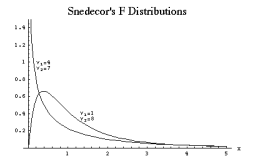
\includegraphics[width=.5\textwidth]{./chaps/23sec/images/2Snedecor_F_distribution.png}
	\end{center}
	\caption{Shape of the graph of $F$-distribution for various degrees of freedom.}
	\label{fig:23sec_F_distribution}
\end{figure}
\paragraph{Properties}
\subparagraph{Expected value and Variance}
$X\hookrightarrow F(\nu_{{1},nu_{2}})\Rightarrow$
$$
E(X) = 
\left\{
\begin{array}{ll}
	\frac{nu_{2}}{nu_{2}-2} & \mbox{if }\nu_{2}\geq 3 \\
	DNE &\mbox{if }\nu_{2}\in\inter{1}{2}
\end{array}
\right.
$$
\begin{center}
	And
\end{center}
$$
V(X) = 
\left\{
\begin{array}{ll}
	\frac{2\nu_{2}^{2}(\nu_{1}+\nu_{2}-2)}{\nu_{1}(\nu_{2}-2)^{2}(\nu_{2}-4)} & \mbox{if }\nu_{2}\geq 5 \\
	DNE &\mbox{if }\nu_{2}\in\inter{1}{4}
\end{array}
\right.
$$
\subparagraph{Inverse}
$X\hookrightarrow F(\nu_{1},\nu_{2})\Rightarrow \frac{1}{X}\hookrightarrow F(\nu_{2},\nu_{1})$\\
\subparagraph{Chi-squared and $F$-distributions}
$
\begin{cases}
	U\hookrightarrow\chi_{2}(\nu_{1})\\
	V\hookrightarrow\chi_{2}(\nu_{2})\\
	U\& V independent
\end{cases}
\Rightarrow
\dfrac{\frac{U}{\nu_{1}}}{\frac{V}{\nu_{2}}}\hookrightarrow F(\nu_{1},\nu_{2})
$
\subparagraph{Quotient of Inverses}
Let $X\hookrightarrow N(\mu_{1},\sigma_{1}^{2})\text{ and }\prth{X}{i}{1}{n}$ be a random sample of size $n$ from the population $X$.
Let $Y\hookrightarrow N(\mu_{2},\sigma_{2}^{2})\text{ and }\prth{Y}{i}{1}{m}$ be a random sample of size $n$ from the population $Y$.
$$
\dfrac{\frac{S_{1}^{2}}{\sigma_{1}^{2}}}{\frac{S_{2}^{2}}{\sigma_{2}^{2}}} \hookrightarrow F(n-1, m-1)
$$
where $S_{1}^{2}$, and $S_{2}^{2}$ denote the sample variances of the
first and second sample, respectively.

